\documentclass{article}

% Images
\usepackage{float}
\usepackage{graphicx}
\usepackage{subcaption}

% Item Enumeration
\usepackage{enumitem}
% Easy List
\usepackage[ampersand]{easylist}

% References
\usepackage{hyperref}

\title{Identificación y Control Neuronal}

\author{
  Pablo Acereda García\\
  Department of Computer Science\\
  University of Alcala\\
  28805 - Alcalá de Henares, Madrid, Spain \\
  \texttt{pablo.acereda@edu.uah.es} \\
  %% examples of more authors
   \And
  Laura Pérez Medeiro\\
  Department of Computer Science\\
  University of Alcala\\
  28805 - Alcalá de Henares, Madrid, Spain \\
  \texttt{l.perezm@edu.uah.es} \\
  %% \AND
  %% Coauthor \\
  %% Affiliation \\
  %% Address \\
  %% \texttt{email} \\
  %% \And
  %% Coauthor \\
  %% Affiliation \\
  %% Address \\
  %% \texttt{email} \\
  %% \And
  %% Coauthor \\
  %% Affiliation \\
  %% Address \\
  %% \texttt{email} \\
}

\begin{document}

% Title
\maketitle

% This page has been left blank intentionally
\newpage
\vspace*{\fill}
 \begin{center}
This page has been intentionally left blank
 \end{center}
\vspace*{\fill}
\newpage

% Table of contents
\tableofcontents

\newpage

\section{Ejercicio 1. Perceptron}

El Perceptron es una función de tipo lineal, que puede resultar indicada cuando
solo hay 2 clases dentro del conjunto de datos. Por este mismo motivo, este tipo
de red neuronal no es perfectamente funcional cuando hay diferentes clases (en
este caso 4).

\begin{figure}[H]
 \centering
 \begin{subfigure}{0.45\textwidth}
  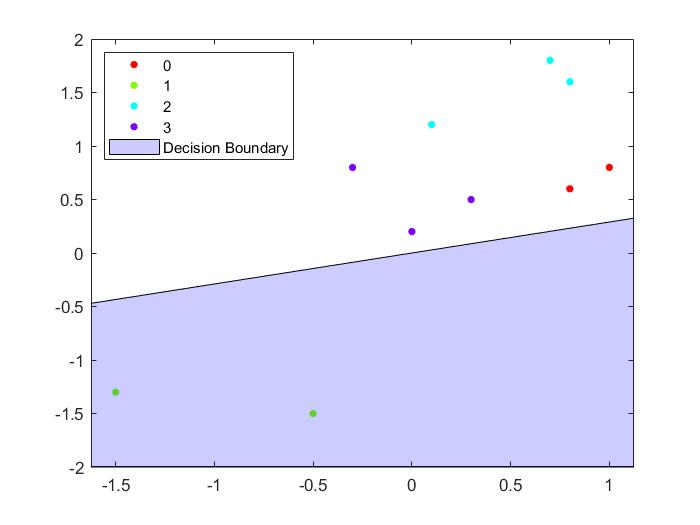
\includegraphics[width=0.9\linewidth]{../images/I_ex1_basicData.jpg}
  \caption{Datos Originales}
 \end{subfigure}
 \begin{subfigure}{0.45\textwidth}
  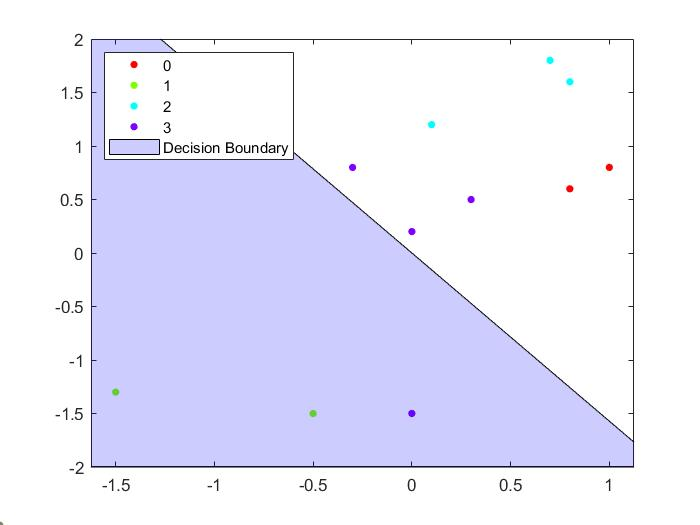
\includegraphics[width=0.9\linewidth]{../images/I_ex1_extendedData.jpg}
  \caption{Datos Extendidos}
 \end{subfigure}
\end{figure}

\section{Ejercicio 2. Aproximación de funciones}

En todos los casos, y con los diferentes métodos de entrenamiento, el
incrementar el tamaño de la capa oculta implica una mayor precisión, número de
iteraciones para completar el proceso y un pequeño incremento del tiempo de
procesado.

En cuanto a las funciones de entrenamiento, se han empleado:

\begin{description}
\item [trainbr] Bayesan Regularization
\item [trainrp] Resilient Backpropagation
\item [trainoss] One Step Secant
\item [traingd] Gradient Descent
\end{description}

\begin{figure}[h]
 \centering
 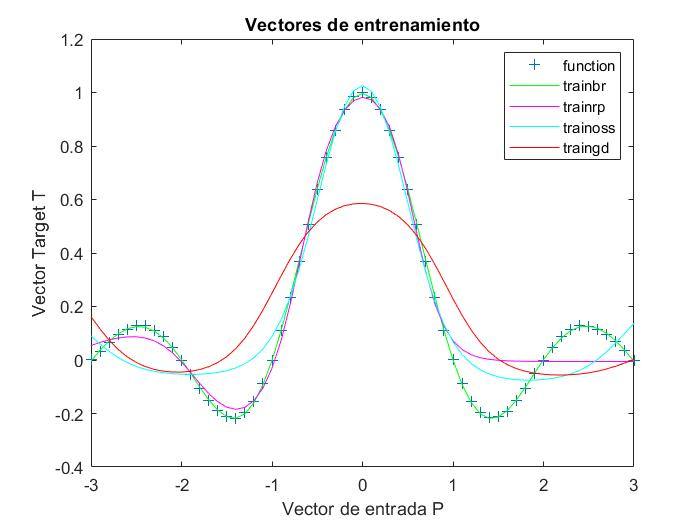
\includegraphics[width=0.8\textwidth]{../I_ex2/training_functions.jpg}
 \caption{Funciones de entrenamiento empleadas.} 
 \label{tf}
\end{figure}

Cambiar la función de entrenamiento puede dar resultados completamente
diferentes. Como se observa en \hyperref[tf]{\ref{tf}} emplear diferentes
funciones puede afectar al tiempo de entrenamiento; al número de iteraciones
(siendo en este caso \textit{traingd} la más costosa); y a la precisión de los
valores obtenidos (siendo \textit{trainbr} la más precisa).

\end{document}
